Im Folgenden werden die Einzelheiten zum Betrieb des Prototypen beschrieben und dienen gleichzeitig als Dokumentation für die zukünftige Entwicklung und Administration des Systems.

\subsection{Nötige Einstellungen bei Slack}
Da der Slackbot als virtueller Nutzer in Slack laufen soll, benötigt dieser eine Verbindung zu entsprechenden Workspace in Slack. Dazu ist vom Administrator/Entwickler ein Slack-Token zu generieren.
Dieser Slack-Token kann unter \url{https://my.slack.com/apps/A0F7YS25R-bots} durch Hinzufügen einer neuen Hubot-Konfiguration generiert werden. Dabei muss der anlegende Nutzer bereits ein Konto bei Slack haben und bereits in dem Workspace registriert sein, in dem der Bot laufen soll.
Nach dem in \autoref{img:hubot-int} erscheinenden Dialog zur Eingabe des Namens für den Bot wird ein eindeutiger Token generiert und angezeigt, dieser wird für die weitere Installation benötigt und beginnt mit \textit{xoxb-}.

\begin{figure}[H]
    \centering
    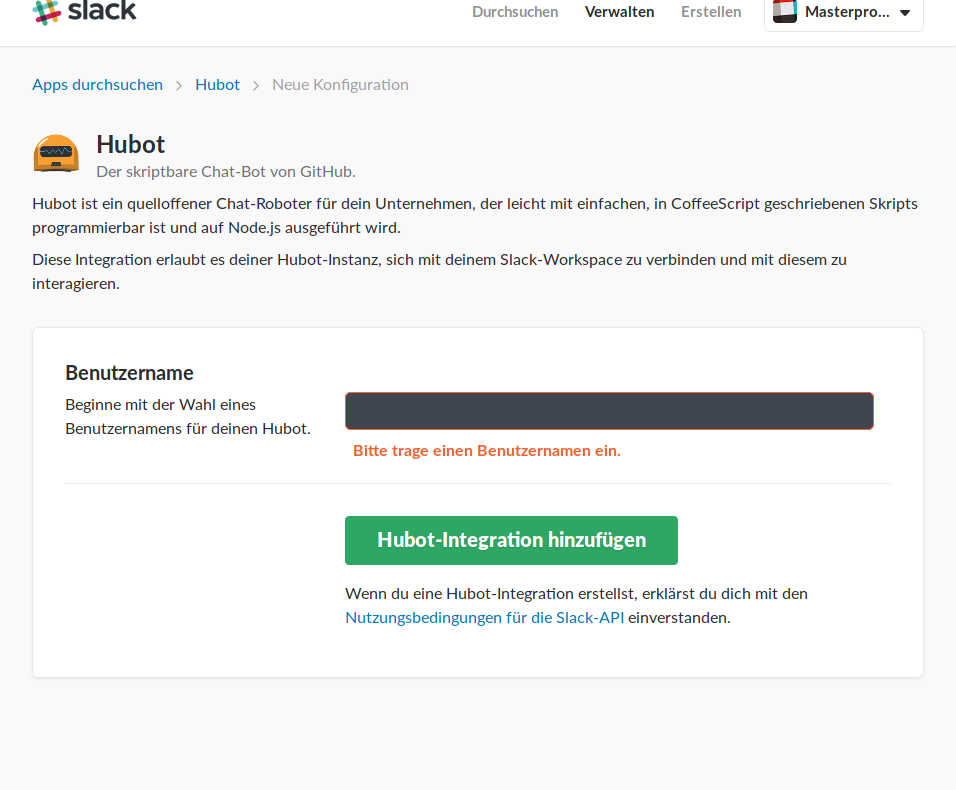
\includegraphics[width=0.8\textwidth]{img/hubot-int.png}
    \caption{Seite zum Anlegen einer neuen Bot-Konfiguration}
    \label{img:hubot-int}
\end{figure}

\subsection{Starten der lokalen Umgebung}
Nach Abruf des Quellcodes von \url{https://github.com/ohli/steckerbot} (über \verb+git clone+ oder Herunterladen des Archivs) befinden sich die Dateien im Ordner \textit{docker} mit folgenden Dateien:

\begin{verbatim}
├── abfragen.sql
├── bin
├── build-docker-image.sh
├── db-data
├── docker-compose.yml
├── Dockerfile
├── external-scripts.json
├── generate_config.sh
├── node_modules
├── package.json
├── scripts
├── steckerbot.env
\end{verbatim}

Die Umgebung wird dynamisch aus zwei Docker-Containern aufgebaut die mittels docker-compose verknüpft werden. Alle vom Standard abweichenden Einstellungen werden über die \verb+steckerbot.env+ definiert, welche über den Aufruf der \verb+generate_config.sh+ generiert werden kann. Beim Aufruf wird automatisch ein Passwort für den MySQL-Rootnutzer generiert sowie weitere Umgebungsvariablen gesetzt. Dies ist nur für Testzwecke vorgesehen und ist im produktiven Betrieb durch ein selbst gewähltes Passwort zu ersetzen. Aktuell liegen die Passwörter im Klartext in der .env-Datei vor, was durch den Einsatz von z.B. Docker Secrets\footnote{\url{https://docs.docker.com/engine/reference/commandline/secret/}} vermieden werden sollte.

\subsection{Anpassen der Umgebungsvariablen}

\subsection{Beispielbefehle}

\subsection{Besonderheiten \& Best Practices}
